
% \documentclass{article}
% % User defined commands
% 
%%
%% Custom Hyphenations
%%
%%
\hyphenation{cross-talk au-di-tory adap-t-a-tion phe-nom-en-o-lo-g-i-cal
  syn-a-pse co-inc-id-ence Tub-er-culo-vent-ral glyc-in-ergic psycho-phys-ical
  asym-met-ric ex-plor-at-ory pot-as-sium op-ti-mi-sa-tion au-di-t-ory system
  Neuro-in-for-mat-ics mar-g-in-al par-a-m-eters Rh-ode Neu-ro-fit-ter
  elec-tro-phys-io-log-i-cal in-fer-ring the con-nec-tiv-i-ty with-in
  non-lin-ear ap-pr-oa-ch-es stel-late mi-cro-cir-cuit show-ing synap-tic
  in-ter-ac-tion iso-lam-inar pop-u-la-tion evo-l-ved com-part-ment
  con-duc-tance mod-els Hod-g-kin Hux-l-ey gluta-m-at-er-gic gen-o-mes
  Theu-nis-sen re-sp-on-se co-inc-id-ence det-e-ctor exp-eri-men-tal
  ac-cu-mu-lated neu-ro-science cre-ate de-tailed ex-ten-sively stud-ied
  In-tra-cel-lu-lar neur-rons in-tra-cel-lu-lar in-ves-ti-ga-tion se-quen-tial
  de-ter-min-ed cat-e-gor-is-ed im-me-di-ate sen-si-tiv-ity bicu-cu-line
  mul-ti-ple in-hib-it-ory com-mis-sural path-way re-cip-ro-cal fre-quency
  po-si-tion func-tion de-lay prep-a-ra-tions iso-lated oct-o-pus in-sen-si-tive
  Chop-per im-preg-na-tion phys-i-o-log-i-cal ef-fect GABA-er-gic in-puts on-set
  chop-pers pri-mar-ily  gen-er-ate ar-ray gaus-sian ran-dom num-bers
  in-ves-ti-gat-ing im-p-or-tant phys-i-o-log-i-cal mech-a-nisms}
%%
%% Sample custom-configuration
%%
%%   You are encouraged to modify the following section with any of your
%%   own custom commands, packages, etc.
%%

%error 'You should modify this section and remove this error.'

% for URLs
\usepackage{url}

% AMS packages
%\usepackage{amsfonts}
\usepackage{amssymb}
\usepackage[fleqn]{amsmath}   % displayed equations flush left
%\setlength{\mathindent}{0em}
%\usepackage{amsthm}
\usepackage[mathscr]{eucal}

\newcommand{\vect}[1]{\mathbf{#1}}


% Allow equations to break over pages...
\interdisplaylinepenalty=2500
% Command to stop equation breaks
% Note: enclose this in braces when used...
\newcommand{\donotsplitoverpages}{\interdisplaylinepenalty=10000}

%% Graphics
% \ifx\pdftexversion\undefined
%  \usepackage[dvips]{graphicx}
% \else
%  \usepackage[pdftex]{graphicx}
% \fi

%% My Graphics and Hyperlinks stuff
\usepackage{ifpdf}
 \ifpdf
   \pdfoutput=1
   \usepackage[pdftex]{graphicx}  % uncomment if using graphicx
\usepackage[final,          % override "draft" which means "do nothing"
            colorlinks,     % rather than outlining them in boxes
            linkcolor=black, % override truly awful colour choices
            citecolor=black, %   (ditto)
            urlcolor=black,  %   (ditto)
            ]{hyperref}

 \ifx\pdfoutput\undefined \usepackage[ps2pdf,
 bookmarks=true,
 bookmarksnumbered=true,
 breaklinks=true,
            final,          % override "draft" which means "do nothing"
            colorlinks,     % rather than outlining them in boxes
            linkcolor=black, % override truly awful colour choices
            citecolor=black, %   (ditto)
            urlcolor=black,  %   (ditto)
            ]{hyperref}

% \usepackage[pdftex]{hyperref}  % uncomment if using hyperref
%  \usepackage[ps2pdf]{thumbpdf}
 \DeclareGraphicsExtensions{.eps,.bmp}
  \else
 \DeclareGraphicsExtensions{.png,.pdf,.jpg,.JPEG}
  \usepackage{epstopdf}
 %\usepackage[pdftex,bookmarks=true,bookmarksnumbered=true,breaklinks=true]{hyperref}
  \pdfadjustspacing=1
  \usepackage[pdftex]{thumbpdf}
  \fi
 \else
   \usepackage[dvips]{graphicx}  % uncomment if using graphicx
    % comment if not using hyperref
 \usepackage[final,          % override "draft" which means "do nothing"
            colorlinks,     % rather than outlining them in boxes
            linkcolor=black, % override truly awful colour choices
            citecolor=black, %   (ditto)
            urlcolor=black,  %   (ditto)
             ]{hyperref}
 \DeclareGraphicsExtensions{.eps,.bmp}
\fi
% Enable IEEE macros
%\usepackage{IEEEtrantools}

% Use a plain bibliography style
%\bibliographystyle{plain}
% Use the IEEE bibliography style (sorted)
%\bibliographystyle{IEEEtrans}
% Use the IEEE bibliography style (unsorted; order of reference)
%\bibliographystyle{IEEEtran}

% For isolated bibliographies
\usepackage{bibunits}

\usepackage{color}
%\usepackage[noadjust]{cite}
\usepackage{caption}
\usepackage{breakurl} % necessary to break URLs when using LaTeX-> dvips -> Ps2PDF, must be after hyperref

% For cool tables
\usepackage{array}
\usepackage{tabularx}  % automatically adjusts column width in tables
\usepackage{multirow}  % allows entries spanning several rows
\usepackage{colortbl}  % allows coloring tables


% For algorithms
%\usepackage{algorithm}
%\usepackage{algorithmic}

% For cases
\usepackage{sublabel}

% For theroem numbers having the chapter included
%\usepackage{style/chngcntr}

% For cool theorem styles
%\usepackage[amsthm]{ntheorem}
%%\theorembodyfont{\normalfont}
%
%% Theorem definition
%\newtheorem{theorem}{Theorem}
%\counterwithin{theorem}{chapter}
%
%% Corollary definition
%\newtheorem{corollary}{Corollary}
%\counterwithin{corollary}{chapter}
%
%% Result definition
%\newtheorem{result}{Result}
%\counterwithin{result}{chapter}
%
%% Lemma definition
%\newtheorem{lemma}{Lemma}
%\counterwithin{lemma}{chapter}
%
%% Proposition definition
%\newtheorem{proposition}{Proposition}
%\counterwithin{proposition}{chapter}
%
%% Definition definition!
%\newtheorem{definition}{Definition}
%\counterwithin{definition}{chapter}
%
%% Remark definition (no counter?)
%\newenvironment{remark}{\emph{Remark:~}}{}
%
%% Fact definition (no counter?)
%\newenvironment{fact}{\emph{Fact:~}}{}

% (Re)Set the figure path
\newcommand{\setfigurepath}[1]{%
\ifx\figurepath\undefined
	\newcommand{\figurepath}{#1}
\else
	\renewcommand{\figurepath}{#1}
\fi%
}

% Used in the continued list environment below
\newcounter{continuedlist}

% Continued list environment
\newenvironment{continuedlist}{%
	\begin{enumerate}%
		% Space out each item
		\setlength{\itemsep}{1.25em}%
		% Start the enumeration from the previous value
		\setcounter{enumi}{\value{continuedlist}} %
}{ %
  % Save the counter to continue it later
  \setcounter{continuedlist}{\value{enumi}}%
  \end{enumerate}%
  % \vspace{1.25em}% 
  \vspace{1em}%
}

% Spaced out list environment
\newenvironment{spacedoutlist}{%
	\begin{itemize}%
		% Space out each item
		\setlength{\itemsep}{1.25em}%
}{\end{itemize}}


%% My added packages


\usepackage[usenames,dvipsnames]{xcolor}
\definecolor{halfgray}{gray}{0.55}

\usepackage{listings}
\lstset{language=C++,%[LaTeX]Tex,%
    keywordstyle=\color{RoyalBlue},%\bfseries,
    basicstyle=\small\sffamily,
    identifierstyle=\color{NavyBlue},
    commentstyle=\color{Green}\rmfamily,
    stringstyle=\sffamily,
    numbers=left,%none,%
    numberstyle=\scriptsize,%\tiny
    stepnumber=5,
    numbersep=8pt,
    showstringspaces=false,
    breaklines=true,
    %frameround=ftff,
    %frame=single
    %frame=L
    lineskip=-5pt
}


% \lstset{language=Octave,                % choose the language of the code
% basicstyle=\footnotesize,       % the size of the fonts that are used for the code
% numbers=left,                   % where to put the line-numbers
% numberstyle=\footnotesize,      % the size of the fonts that are used for the line-numbers
% stepnumber=2,                   % the step between two line-numbers. If it's 1 each line will be numbered
% numbersep=5pt,                  % how far the line-numbers are from the code
% backgroundcolor=\color{white},  % choose the background color. You must add \usepackage{color}
% showspaces=false,               % show spaces adding particular underscores
% showstringspaces=false,         % underline spaces within strings
% showtabs=false,                 % show tabs within strings adding particular underscores
% frame=single,			% adds a frame around the code
% tabsize=2,			% sets default tabsize to 2 spaces
% captionpos=b,			% sets the caption-position to bottom
% breaklines=true,		% sets automatic line breaking
% breakatwhitespace=false,	% sets if automatic breaks should only happen at whitespace
% lineskip=-5pt  %
% }

\ifx\setcitestyle\undefined
\usepackage[sort,round,authoryear]{natbib}
\setcitestyle{aysep={}} % J Neurophys formatting
\fi

\usepackage{xspace}
\usepackage{rotating}
\usepackage{tikz}
\usepackage{calc}

\newcommand{\hdr}[3]{%
\multicolumn{#1}{|l|}{\color{white}\cellcolor[gray]{0.0}%
\textbf{\makebox[0.05\linewidth][l]{#2}\hspace{0.45\linewidth}\makebox[0pt][c]{#3}}%
%\textbf{\makebox[0pt]{#2}\hspace{0.5\linewidth}\makebox[0pt][c]{#3}}%
}}
 % Nordelie table environment
\newenvironment{ntab}[4]{
\noindent\begin{tabularx}{\linewidth}{#1}\hline 
\multicolumn{#2}{|l|}{\color{white}\cellcolor[gray]{0.0}\textbf{#3\hfill{}{#4}\hfill{}}}
}{
\end{tabularx}
\vspace{1ex}
}



\usepackage[colorinlistoftodos,backgroundcolor=yellow!35,textsize=footnotesize]{todonotes}
\newcommand{\yellownote}[1]{\todo[inline]{#1}}


\usepackage{scrtime}
%\usepackage{mparhack}

%\setlength{\parskip}{0ex} or {1.2ex}
%\setlength{\parindent}{0em} or {0ex}

\usepackage[australian]{babel}

\usepackage{booktabs,ltxtable,ctable,dcolumn}
\newcommand{\otoprule}{\midrule[\heavyrulewidth]}

\usepackage{doipubmed}

% For subfigures
\usepackage{keyval}
\usepackage[config,labelfont={sf,bf}]{subfig}
%\captionsetup[table]{position=top}
%\captionsetup[subtable]{position=top}
%\usepackage[heightadjust=all,valign=t]{floatrow}
%\usepackage{fr-subfig}
%\floatsetup{style=Plaintop}
%\usepackage{subfigure}

\usepackage{lscape}

\newcommand{\code}[1]{\mbox{\normalfont\texttt{#1}}}
\newcommand{\progname}[1]{\mbox{\normalfont\textsf{#1}}}
\newcommand{\figfont}[1]{\large{\textbf{\textsf{#1}}}}


% %% Glossary

% ANF to Golgi
\newcommand{\ANFGLG}{\protect\ensuremath{\mbox{ANF} \to \mbox{GLG}\xspace}}
\newcommand{\HSRGLG}{\protect\ensuremath{\mbox{HSR} \to \mbox{GLG}\xspace}}
\newcommand{\LSRGLG}{\protect\ensuremath{\mbox{LSR} \to \mbox{GLG}\xspace}}
\newcommand{\wANFGLG}{\protect\ensuremath{w_{\ANFGLG}\xspace}}
\newcommand{\wLSRGLG}{\protect\ensuremath{w_{\LSRGLG}\xspace}}
\newcommand{\wHSRGLG}{\protect\ensuremath{w_{\HSRGLG}\xspace}}
\newcommand{\nLSRGLG}{\protect\ensuremath{n_{\LSRGLG}\xspace}}
\newcommand{\nHSRGLG}{\protect\ensuremath{n_{\HSRGLG}\xspace}}
\newcommand{\sANFGLG}{\protect\ensuremath{s_{\ANFGLG}\xspace}}
\newcommand{\sLSRGLG}{\protect\ensuremath{s_{\LSRGLG}\xspace}}
\newcommand{\sHSRGLG}{\protect\ensuremath{s_{\HSRGLG}\xspace}}
\newcommand{\dANFGLG}{\protect\ensuremath{d_{\ANFGLG}\xspace}}

%ANF to D-stellate
\newcommand{\ANFDS}{\protect\ensuremath{\mbox{ANF} \to \mbox{DS}\xspace}}
\newcommand{\HSRDS}{\protect\ensuremath{\mbox{HSR} \to \mbox{DS}\xspace}}
\newcommand{\LSRDS}{\protect\ensuremath{\mbox{LSR} \to \mbox{DS}\xspace}}
\newcommand{\wANFDS}{\ensuremath{w_{\ANFDS}\xspace}}
\newcommand{\wLSRDS}{\protect\ensuremath{w_{\LSRDS}\xspace}}
\newcommand{\wHSRDS}{\protect\ensuremath{w_{\HSRDS}\xspace}}
\newcommand{\nLSRDS}{\protect\ensuremath{n_{\LSRDS}\xspace}}
\newcommand{\nHSRDS}{\protect\ensuremath{n_{\HSRDS}\xspace}}
\newcommand{\dANFDS}{\protect\ensuremath{d_{\ANFDS}\xspace}}
\newcommand{\sANFDSh}{\protect\ensuremath{s^+_{\ANFDS}\xspace}}
\newcommand{\sANFDSl}{\protect\ensuremath{s^-_{\ANFDS}\xspace}}

%ANF to T-stellate
\newcommand{\ANFTS}{\protect\ensuremath{\mbox{ANF} \to \mbox{TS}\xspace}}
\newcommand{\HSRTS}{\protect\ensuremath{\mbox{HSR} \to \mbox{TS}\xspace}}
\newcommand{\LSRTS}{\protect\ensuremath{\mbox{LSR} \to \mbox{TS}\xspace}}
\newcommand{\wANFTS}{\protect\ensuremath{w_{\ANFTS}\xspace}}
\newcommand{\nLSRTS}{\protect\ensuremath{n_{\LSRTS}\xspace}}
\newcommand{\nHSRTS}{\protect\ensuremath{n_{\HSRTS}\xspace}}
\newcommand{\sANFTS}{\protect\ensuremath{s_{\ANFTS}\xspace}}
\newcommand{\dANFTS}{\protect\ensuremath{d_{\ANFTS}\xspace}}

%ANF to Tuberculoventral
\newcommand{\ANFTV}{\ensuremath{\mbox{ANF} \to \mbox{TV}\xspace}}
\newcommand{\HSRTV}{\ensuremath{\mbox{HSR} \to \mbox{TV}\xspace}}
\newcommand{\LSRTV}{\ensuremath{\mbox{LSR} \to \mbox{TV}\xspace}}
\newcommand{\wANFTV}{\ensuremath{w_{\ANFTV}\xspace}}
\newcommand{\nLSRTV}{\ensuremath{n_{\LSRTV}\xspace}}
\newcommand{\nHSRTV}{\ensuremath{n_{\HSRTV}\xspace}}
\newcommand{\sANFTV}{\ensuremath{s_{\ANFTV}\xspace}}
\newcommand{\dANFTV}{\ensuremath{d_{\ANFTV}\xspace}}

%GLG to T-stellate
\newcommand{\GLGTS}{\protect\ensuremath{\mbox{GLG} \to \mbox{TS}\xspace}}
\newcommand{\wGLGTS}{\protect\ensuremath{w_{\GLGTS}\xspace}}
\newcommand{\nGLGTS}{\protect\ensuremath{n_{\GLGTS}\xspace}}
\newcommand{\sGLGTS}{\protect\ensuremath{s_{\GLGTS}\xspace}}
\newcommand{\dGLGTS}{\protect\ensuremath{d_{\GLGTS}\xspace}}
%GLG to D-stellate
\newcommand{\GLGDS}{\protect\ensuremath{\mbox{GLG} \to \mbox{DS}\xspace}}
\newcommand{\wGLGDS}{\protect\ensuremath{w_{\GLGDS}\xspace}}
\newcommand{\nGLGDS}{\protect\ensuremath{n_{\GLGDS}\xspace}}
\newcommand{\sGLGDS}{\protect\ensuremath{s_{\GLGDS}\xspace}}
\newcommand{\dGLGDS}{\protect\ensuremath{d_{\GLGDS}\xspace}}

% % TS to Golgi
% \newcommand{\GLGTS}{\protect\ensuremath{\mbox{GLG} \to \mbox{TS}\xspace}}
% \newcommand{\wTSGLG}{\protect\ensuremath{w_{}}\xspace}}
% \newcommand{\nTSGLG}{\protect\ensuremath{n_{\mbox{TS} \to \mbox{GLG}}\xspace}}
% \newcommand{\sTSGLG}{\protect\ensuremath{s_{\mbox{TS} \to \mbox{GLG}}\xspace}}
% \newcommand{\dTSGLG}{\protect\ensuremath{d_{\mbox{TS} \to \mbox{GLG}}\xspace}}

%TS to D-stellate
\newcommand{\TSDS}{\protect\ensuremath{\mbox{TS} \to \mbox{DS}\xspace}}
\newcommand{\wTSDS}{\protect\ensuremath{w_{\TSDS}\xspace}}
\newcommand{\nTSDS}{\protect\ensuremath{n_{\TSDS}\xspace}}
\newcommand{\sTSDS}{\protect\ensuremath{s_{\TSDS}\xspace}}
\newcommand{\dTSDS}{\protect\ensuremath{d_{\TSDS}\xspace}}
%TS to T-stellate
\newcommand{\TSTS}{\protect\ensuremath{\mbox{TS} \to \mbox{TS}\xspace}}
\newcommand{\wTSTS}{\protect\ensuremath{w_{\TSTS}\xspace}}
\newcommand{\nTSTS}{\protect\ensuremath{n_{\TSTS}\xspace}}
\newcommand{\sTSTS}{\protect\ensuremath{s_{\TSTS}\xspace}}
\newcommand{\dTSTS}{\protect\ensuremath{d_{\TSTS}\xspace}}

%TS to Tuberculoventral
\newcommand{\TSTV}{\protect\ensuremath{\mbox{TS} \to \mbox{TV}\xspace}}
\newcommand{\wTSTV}{\protect\ensuremath{w_{\TSTV}\xspace}}
\newcommand{\nTSTV}{\protect\ensuremath{n_{\TSTV}\xspace}}
\newcommand{\sTSTV}{\protect\ensuremath{s_{\TSTV}\xspace}}
\newcommand{\dTSTV}{\protect\ensuremath{d_{\TSTV}\xspace}}

% DS to Golgi
\newcommand{\DSGLG}{\protect\ensuremath{\mbox{DS} \to \mbox{GLG}\xspace}}
\newcommand{\wDSGLG}{\protect\ensuremath{w_{\DSGLG}\xspace}}
\newcommand{\nDSGLG}{\protect\ensuremath{n_{\DSGLG}\xspace}}
\newcommand{\sDSGLG}{\protect\ensuremath{s_{\DSGLG}\xspace}}
\newcommand{\dDSGLG}{\protect\ensuremath{d_{\DSGLG}\xspace}}

% %DS to D-stellate
% \newcommand{\DSDS}{\protect\ensuremath{\mbox{DS} \to \mbox{DS}\xspace}}
% \newcommand{\wDSDS}{\protect\ensuremath{w_{\DSDS}\xspace}}
% \newcommand{\nDSDS}{\protect\ensuremath{n_{\DSDS}\xspace}}
% \newcommand{\sDSDS}{\protect\ensuremath{s_{\DSDS}\xspace}}
% \newcommand{\dDSDS}{\protect\ensuremath{d_{\DSDS}\xspace}}

%DS to T-stellate
\newcommand{\DSTS}{\protect\ensuremath{\mbox{DS} \to \mbox{TS}\xspace}}
\newcommand{\wDSTS}{\protect\ensuremath{w_{\DSTS}\xspace}}
\newcommand{\nDSTS}{\protect\ensuremath{n_{\DSTS}\xspace}}
\newcommand{\sDSTS}{\protect\ensuremath{s_{\DSTS}\xspace}}
\newcommand{\dDSTS}{\protect\ensuremath{d_{\DSTS}\xspace}}

%DS to Tuberculoventral
\newcommand{\DSTV}{\protect\ensuremath{\mbox{DS} \to \mbox{TS}\xspace}}
\newcommand{\wDSTV}{\protect\ensuremath{w_{\DSTV}\xspace}}
\newcommand{\nDSTV}{\protect\ensuremath{n_{\DSTV}\xspace}}
\newcommand{\sDSTV}{\protect\ensuremath{s_{\DSTV}\xspace}}
\newcommand{\dDSTV}{\protect\ensuremath{d_{\DSTV}\xspace}}
\newcommand{\oDSTV}{\protect\ensuremath{o_{\DSTV}\xspace}}

% TV to Golgi
\newcommand{\TVGLG}{\protect\ensuremath{\mbox{TV} \to \mbox{GLG}\xspace}}
\newcommand{\wTVGLG}{\protect\ensuremath{w_{\TVGLG}\xspace}}
\newcommand{\nTVGLG}{\protect\ensuremath{n_{\TVGLG}\xspace}}
\newcommand{\sTVGLG}{\protect\ensuremath{s_{\TVGLG}\xspace}}
\newcommand{\dTVGLG}{\protect\ensuremath{d_{\TVGLG}\xspace}}

%TV to D-stellate
\newcommand{\TVDS}{\protect\ensuremath{\mbox{TV} \to \mbox{DS}\xspace}}
\newcommand{\wTVDS}{\protect\ensuremath{w_{\TVDS}\xspace}}
\newcommand{\nTVDS}{\protect\ensuremath{n_{\TVDS}\xspace}}
\newcommand{\sTVDS}{\protect\ensuremath{s_{\TVDS}\xspace}}
\newcommand{\dTVDS}{\protect\ensuremath{d_{\TVDS}\xspace}}

%TV to T-stellate
\newcommand{\TVTS}{\protect\ensuremath{\mbox{TV} \to \mbox{TS}\xspace}}
\newcommand{\wTVTS}{\protect\ensuremath{w_{\TVTS}\xspace}}
\newcommand{\nTVTS}{\protect\ensuremath{n_{\TVTS}\xspace}}
\newcommand{\sTVTS}{\protect\ensuremath{s_{\TVTS}\xspace}}
\newcommand{\dTVTS}{\protect\ensuremath{d_{\TVTS}\xspace}}

%TV to Tuberculoventral
\newcommand{\TVTV}{\protect\ensuremath{\mbox{TV} \to \mbox{TV}\xspace}}
\newcommand{\wTVTV}{\protect\ensuremath{w_{\TVTV}\xspace}}
\newcommand{\nTVTV}{\protect\ensuremath{n_{\TVTV}\xspace}}
\newcommand{\sTVTV}{\protect\ensuremath{s_{\TVTV}\xspace}}
\newcommand{\dTVTV}{\protect\ensuremath{d_{\TVTV}\xspace}}


%Other common symbols
\newcommand{\GABAa}{\ensuremath{\mbox{GABA}_\mbox{A}}}

% \usepackage[margin=0.2in]{geometry} % get enough space on page

% \usepackage{tabularx}  % automatically adjusts column width in tables
% \usepackage{multirow}  % allows entries spanning several rows
% \usepackage{colortbl}  % allows coloring tables
% % \usepackage{natbib}
% % \usepackage[fleqn]{amsmath}   % displayed equations flush left
% % \setlength{\mathindent}{0em}

% % use Helvetica for text, Pazo math fonts
% \usepackage{mathpazo}
% \usepackage[scaled=.95]{helvet}
% \renewcommand\familydefault{\sfdefault}

% \renewcommand\arraystretch{1.2}  % slightly more space in tables

% \pagestyle{empty}  % no header of footer

% \hdr{ncols}{label}{title}
% 
% Typeset header bar across table with ncols columns
% with label at left margin and centered title
% 


% \graphicspath{{/media/data/Work/cnstellate/Responses2/}{/media/data/Work/cnstellate/}}


%\begin{document}

%%%%%%%%%%%%%%%%%%%%%%%%%%%%%%%%%%%%%%%%%%%%% 
%%%%%%%%%%%%%%%%%%%%%%%%%%%%%%%%%%%%%%%%%%%%% 
%%%%%%%%%%%%%%%%%%%%%%%%%%%%%%%%%%%%%%%%%%%%% 

\section{T~stellate cell units}


\subsection{Background}
\label{sec:backgrTS}


\begin{itemize}
\item histology staining
\begin{itemize}
\item multipolar (Nissl staining) and stellate (Golgi impregnation) \citep{Osen:1969,BrawerMorestEtAl:1974,Lorente:1981}
\end{itemize}
\item axonal projections
\begin{itemize}
\item \textbf{T} trapezoid body or ventral acoustic stria (T stellate), and \textbf{D} dorsal acoustic stria (D stellate) \citep{OertelWuEtAl:1990}
\item T stellates project locally in VCN and deep layer of DCN $\rightarrow$ match Chopper \citep{RhodeOertelEtAl:1983,SmithRhode:1989}
\item D stellate projections wide in VCN,DCN and cCN $\rightarrow$ match OnC  \citep{SmithRhode:1989}
\end{itemize}
\item somatic innervation: type 1 (few somatic) type II (many somatic and dendritic) \citep{Cant:1981}
\item anatomical and physiological: \citet{SmithRhode:1989}
\begin{itemize}
\item T stellate $\rightarrow$ type 1 $\rightarrow$ chopping PSTH
\item D stellate $\rightarrow$ type 2 $\rightarrow$ OnC PSTH
\end{itemize}
\item Chopper subdivision:
\begin{itemize}
\item sustained and transient (no evidence for anatomical differences in T\~{}stellate cells)
\end{itemize}
\item dendritic differences \citep{DoucetRyugo:1997,DoucetRyugo:2006}
\begin{itemize}
\item planar (T) and radial (D)
\end{itemize}
\end{itemize}

\subsection{Acoustic Response of T stellate cells}
\label{sec-1_2}



\begin{itemize}
\item regular, tonic response to tones \citep{RhodeOertelEtAl:1983,SmithRhode:1989,BlackburnSachs:1989}
\item ``Chopping'' precise regular timing that degrades throughout stimulus\citep{YoungRobertEtAl:1988,BlackburnSachs:1989}
\begin{itemize}
\item sustained (70\%) $\rightarrow$ constant rate, ISI histogram sharp, CV \textless 0.3, CV constant
\item transient (30\%) $\rightarrow$ rate decreases, CV starts below 0.3 then varies
\end{itemize}
\item Inhibition
\begin{itemize}
\item Gly, GABA tuned on frequency to reduce peak excitation \citep{CasparyBackoffEtAl:1994}
\item inhibitory side bands mainly D stellate \citep{FerragamoGoldingEtAl:1998a} but periolivary also contribute \citep{AdamsWarr:1976,Adams:1983,ShoreHelfertEtAl:1991,OstapoffBensonEtAl:1997}
\end{itemize}
\end{itemize}
\citep{PalombiCaspary:1992,RhodeSmith:1986,NelkenYoung:1994,PaoliniClareyEtAl:2005,PaoliniClareyEtAl:2004}  

\begin{itemize}
\item sustained firing despite AN adaptation
\begin{itemize}
\item signals the sound intensity consistently, hence precise level information
\item Phasic also do level, but tonic suits encoding of spectrum across population since encoding the peaks and valleys is relatively independent of time after onset of sound \citep{BlackburnSachs:1990,May:2003,MayPrellEtAl:1998,MaySachs:1998}
\item suits encong of envelope of sounds, important for speech (envelops under 50 Hz \citep{ShannonZengEtAl:1995}
\end{itemize}
\item AM coding in choppers encoded over wide range of intensities \citep{RhodeGreenberg:1994,FrisinaSmithEtAl:1990}
\begin{itemize}
\item other work in Am coding by CN neurons  \citep{Moller:1972,Moller:1974a,Moller:1974,MooreCashin:1974,Frisina:1984,PalmerWinterEtAl:1986,KimRhodeEtAl:1986,WinterPalmer:1990a,Palmer:1990,PalmerWinter:1992,FrisinaSmithEtAl:1990a,Frisina:1983,GorodetskaiaBibikov:1985,RhodeGreenberg:1994,ShofnerSheftEtAl:1996,FrisinaKarcichEtAl:1996,DAngeloSterbingEtAl:2003,Aggarwal:2003}
\end{itemize}
\item phasic firing in AN maintained by bushy
\begin{itemize}
\item phasic info important: enhances formant transitions, and provides accurate information about the location of sound sources even in reverberant environments, critical in hearing \cite{DelgutteKiang:1984,DelgutteKiang:1984a,DelgutteKiang:1984b,DelgutteKiang:1984c,DelgutteKiang:1984d,DavoreIhlefeldEtAl:2009}
\end{itemize}
\end{itemize}
\subsection{Mechanisms making phasic input tonic}
\label{sec-1_3}


   steady depolarising current shows intracellular ability to be tonic \cite{Oertel:1983,OertelWuEtAl:1988} BUT - how does the input remain stable given AN adaptation?


\begin{enumerate}
\item selective processing of HSR and LSR input
\begin{enumerate}
\item feed-forward excitation in TS cells
\begin{itemize}
\item axon collaterals in local isofrequency (most cells in PVCN are TS cells)
\end{itemize}
\item co-activation of phasic inhibition
\begin{itemize}
\item DS inhibition ispi and contralaterally
\begin{itemize}
\item onset inhibition strongest, affecting TS cells after first spike
\item broad tuning sharpens FSL
\end{itemize}
\item TV sharply tuned inhibition (Ferr98)
\begin{itemize}
\item TV response variable and non-monotonic
\item \citep{Rhode:1999}  labelled TV cells phasic in aneasthetised cats
\item unanesthetised cats and gerbils are phasic or tonic  \citep{DingVoigt:1997,ShofnerYoung:1985}
\end{itemize}
\item Others - Glycine from ipsi periolivary region, GABA from both
          periolivary regions \citep{AdamsWarr:1976,ShoreHelfertEtAl:1991,OstapoffBensonEtAl:1997}
\end{itemize}
\item Absense of LT potassium in TS
\begin{itemize}
\item labelled \citep{ManisMarx:1991,BalOertel:2001,FerragamoOertel:2002,CaoShatadalEtAl:2007}
\item unlabelled \citep{RothmanManis:2003,RothmanManis:2003a,RothmanManis:2003b,Rothman:1999}
\end{itemize}
\item Activation of NMDA
\begin{itemize}
\item \citep{CaoOertel:2010} shows TS cells activate large currents through NMDA receptors
\item NMDA longer lasting, reducing phasic nature of input
\end{itemize}
\item Little synaptic depression
\begin{itemize}
\item SD less tahn bushy and octopus \citep{WuOertel:1987,ChandaXu-Friedman:2010,CaoOertel:2010}
\item excitation of TS adapts less than other VCN neurons
\end{itemize}
\end{enumerate}
\end{enumerate}
\subsection{Mechanisms of tonic firing obscure temporal features}
\label{sec-1_4}



\begin{itemize}
\item sFSL largest in TS of core VCN units by 1 msec $\rightarrow$ onset inhibition + longer integration time \citep{GisbergenGrashuisEtAl:1975,GisbergenGrashuisEtAl:1975a,GisbergenGrashuisEtAl:1975b,YoungRobertEtAl:1988,PaoliniClareyEtAl:2004}
\item integration window longest for choppers \citep{McGinleyOertel:2006}
\item inhibition from high CF units alters FSL to tones \citep{Wickesberg:1996}
\item Onset: Volley of Excitation + feedforward excitation + DS inhibition
\item After onset: Phasic excitation + feedforward excitation + NMDA activation + TV inhibition (+ small DS inhibition) + GABA inhibition = stable excitation but loss of temporal features
\end{itemize}

\subsection{Neuromodulatory effects in T stellate cells}
\label{sec-1_5}



\begin{itemize}
\item sensitive to neuromodulatory currents \citep{FujinoOertel:2001}
\begin{itemize}
\item high input resistance $\rightarrow$ amplify small current inputs \citep{FujinoOertel:2001}
\item no LKT in TS,  LKT makes bushy and optopus insensitive to steady currents \citep{OertelFujino:2001,McGinleyOertel:2006}
\item Ih higher in TS \& activated more at lower potentials than in bushy and octopus, so that it is less active at rest
\item high resistance $\rightarrow$ greater voltage changes in small modulating current $\rightarrow$ Ih can be modulated by G-protein coupled receptors, hence making TS more excitable when Ih activated \citep{RodriguesOertel:2006}
\end{itemize}
\end{itemize}

\begin{enumerate}
\item Driving inputs
\end{enumerate}
Proximal dendrites and at the soma:

\begin{itemize}
\item ANF provide glutamatergic excitation for T stellates  \citep{Cant:1981,FerragamoGoldingEtAl:1998a,Alibardi:1998a}
\begin{itemize}
\item only 5 or 6 in mice \citep{FerragamoGoldingEtAl:1998a,CaoOertel:2010}
\end{itemize}
\item Recurrent excitation from other T stellate cells \citep{FerragamoGoldingEtAl:1998a}
\item Glycine from DS cells \citep{FerragamoGoldingEtAl:1998a}
\item Glycine from TV cells \citep{WickesbergOertel:1990,ZhangOertel:1993b}
\item Neuromodulatory
\end{itemize}
     No signs of PSP or PSCs hence distal or G-protein coupled, effects on time-course minimal
     
a. Golgi cells (GABA)

\begin{itemize}
\item no IPSPs or IPSCs but presence of GABAa receptors and response changes to bicuculine \citep{WuOertel:1986,OertelWickesberg:1993,FerragamoGoldingEtAl:1998a}
\item dend filter obscures PSPs
\item Golgi cells are GABAergic and lie within the granule cell domains around the VCN and terminate near the fine distal dendrites of T stellate cells
\end{itemize}
b. Periolivary cells (GABA + GAD - glutamic acid decarboxylase) 

\begin{itemize}
\item observed in PVCN close to TS \citep{AdamsMugnaini:1987}
\item GAD effectively Glycine \citep{GoldingOertel:1997}
\item can also arise from GABAergic neurons in ipsi LNTB and DM Periolivary
\end{itemize}
c. VNTB cells (ACh)

\begin{itemize}
\item collateral branches of OC go to GCD \citep{MellottMottsEtAl:2011,SherriffHenderson:1994,OsenRoth:1969}
\item TS have nicotinic and muscarinic ACh receptors \citep{FujinoOertel:2001}
\item ACh input to TS, together with OC-cochlea, enhances spectral peaks in noise  \citep{FujinoOertel:2001}
\end{itemize}
d. NE and 5HT

\begin{itemize}
\item Raphe nuclei (5HT)
\item Locus coeruleus Peribrachial cells (NE)
\item both terminate in PVCN \citep{KlepperHerbert:1991,Thompson:2003,ThompsonLauder:2005,Thompson:2003a,ThompsonWiechmann:2002,BehrensSchofieldEtAl:2002,ThompsonThompson:2001,ThompsonThompson:2001a,ThompsonMooreEtAl:1995,ThompsonThompsonEtAl:1994}
\item both increase firing in T stellates \citep{OertelWrightEtAl:2010} in presence of glut and gly blockers -> hence act on post synapse (TS cells)
\item both G-protein coupled, both act on either pre or post synaptic cells
\item NE affects probability of release at calyx of Held
\item NE increases firing rate of choppers \citep{KosslVater:1989,Ebert:1996}
\item 5HT excites or inhibits choppers \emph{in vivo} \citep{EbertOstwald:1992}
\end{itemize}
\subsection{Major ascending output}
\label{sec-1_6}


\begin{itemize}
\item review \citep{DoucetRyugo:2006}
\end{itemize}

TS cell axons exit the CN through the trapezoidal body, cross the midline and ultimately terminate in the cIC \citep{Adams:1979}


\begin{itemize}
\item Collaterals: local, DCN, LSO cVNTB cVNLL \citep{Warr:1969,SmithJorisEtAl:1993,Thompson:1998,DoucetRyugo:2003}
\item Deep DCN (bulk of acoustic input?)
\item in mice TS terminals > ANF \citep{CaoMcGinleyEtAl:2008}
\item on CF \citep{SmithRhode:1989,FriedlandPongstapornEtAl:2003,DoucetRyugo:1997}
\item DCN review \citep{OertelYoung:2004}
\item LSO excitation
\item TS project to LSO \citep{Thompson:1998,DoucetRyugo:2003,ThompsonThompson:1991a}
\item LSO detect interauriculal intensity differences primarily from ipsi Bushy cells and contra MNTB (inhib)
\item OC feedback
\end{itemize}

a. MOC: cVNTB excitation 

\begin{itemize}
\item involved in efferent feedback loop, ACh-ergic MOC neurons TS synapses in cVNTB \citep{WarrBeck:1996,Warr:1992,Warr:1982,VeneciaLibermanEtAl:2005,ThompsonThompson:1991,SmithJorisEtAl:1993}
\item feedback direct to TS is positive, but efferent MOC-OHC-ANF reduces activation of ANF \citep{WarrenLiberman:1989,WiederholdKiang:1970}
\item other \citep{RobertsonMulders:2000,WinterRobertsonEtAl:1989}
\end{itemize}

b. LOC

\begin{itemize}
\item TS terminate in vicinity of LOC neurons \citep{Warr:1982,ThompsonThompson:1988,ThompsonThompson:1991,DoucetRyugo:2003}
\item feedback through LOC $\rightarrow$ cochlea $\rightarrow$ ANF loop $\rightarrow$ TS affect/regulate response of LOC. hence ANF.
\item LOC balance inputs from both ears \citep{DarrowMaisonEtAl:2006}
\end{itemize}

c. VNLL

\begin{itemize}
\item The functional consequences of these direct and indirect connections with TS cells with the IC are not well understood
\end{itemize}
% %\subsection{TS cells in birds}
% \label{sec-1_7}


% VCN analog is the \emph{nucleus angularis}
% %\subsection{Summary}
% \label{sec-1_8}


% As a population, T stellate cells encode the spectrum of sounds. They
% receive acoustic input from the auditory nerve fibers. Several
% mechanisms contribute to that transformation: Feed-forward excitation
% through other T stellate cells, co-activation of excitation and
% inhibition, reduction in synaptic depression, and the amplification of
% excitatory synaptic current over time through NMDA receptors. They
% deliver that information to nuclei that make use of spectral
% information.  T stellate cells terminate in the DCN, to olivocochlear
% efferent neurons, to the lateral superior olive, to the contralateral
% inferior colliculus. These targets use spectral information to
% localize sounds, to adjust the sensitivity of the inner ear, and to
% recognise and understand sounds. Birds also process sounds through
% neurons that resemble T stellate cells in their projections and also
% in their cellular properties, attesting to the fundamental importance
% that T stellate-like cells have for hearing in vertebrates.




% \citep{Oertel:2010}
% - naming: 
% --multipolar (Nissl staining) and stellate (Golgi impregnation) Osen, Brawer, Lorente
% - axonal projections
% -- *T*rapezoid and *D*orsal  (Oertel et al 90)
% -- T stellates project locally in VCN and deep layer of DCN
% - somatic innervation: type 1 (few somatic) type II (many somatic and dendritic) Cant
% - anatomical and physiological: Smith and Rhode
% -- type 1 -> chopping PSTH
% -- type 2 -> OnC PSTH
% - Chopper subdivision:
% -- sustained and transient (no evidence for anatomical differences in T~stellates)



The work by Tony Paolini, Janine Clarey, Karina Needham and others at the Royal
Victorian Eye and Ear Hospital, were pivotal in developing my network model of
the cochlear nucleus, in particular my interest in chopper units and T~stellate
cells.  Figure~\ref{fig:PaoliniAIV} shows the intracellular acoustic
classification of chopper units in the rat into three distinct types
\citep{PaoliniClareyEtAl:2005}: CS chopper sustained, and two transient choppers
CT1 and CT2.  This work expands on the extracellular classification by
\citep{BlackburnSachs:1989} into slowly or transiently adapting and sustained
choppers in cats. The intracellular traces in Figure~\ref{fig:PaoliniAIV} will
form the basis for the optimisation routine of T~stellate cell model


\begin{figure}[htb]
  \centering
\subfloat[Chopper Sustained]{\resizebox{0.3\textwidth}{!}{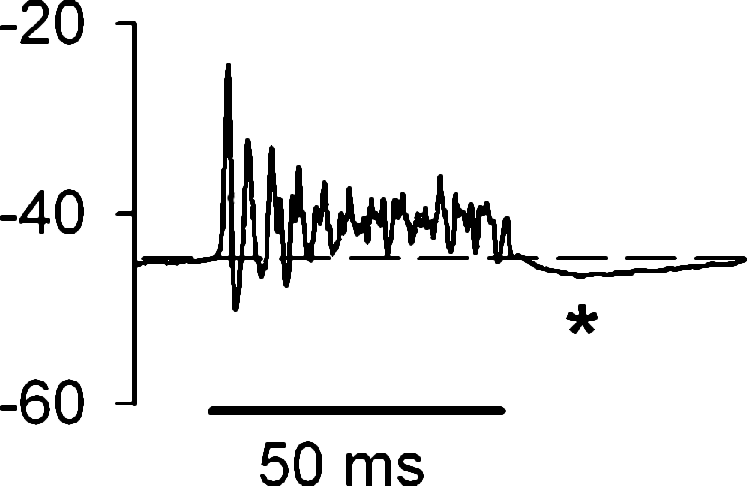
\includegraphics{TStellate/CS-01-864-004}}}\hfill%\quad%
\subfloat[Chopper Transient 1]{\resizebox{0.3\textwidth}{!}{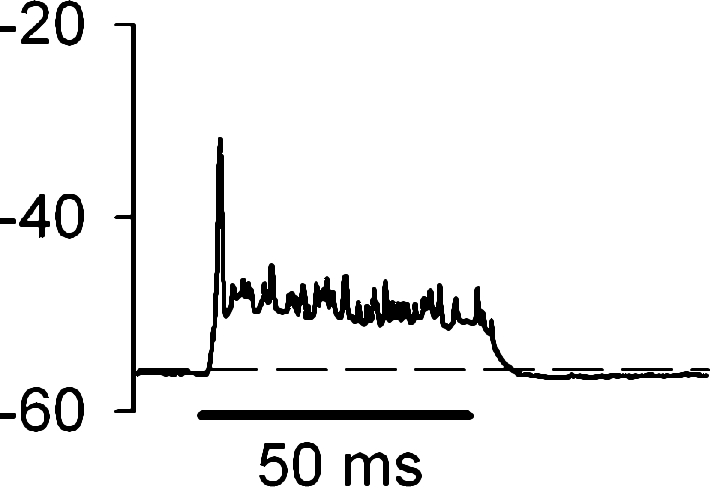
\includegraphics{TStellate/CT1-01-857-007}}}\hfill%\\
\subfloat[Chopper Transient 2]{\resizebox{0.3\textwidth}{!}{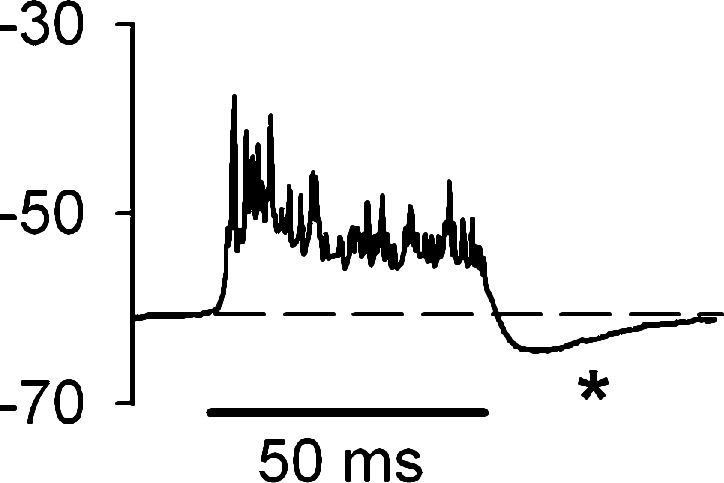
\includegraphics{TStellate/CT2-01-305-014}}}%\quad%
%\subfloat[Onset Chopper]{\resizebox{0.35\textwidth}{!}{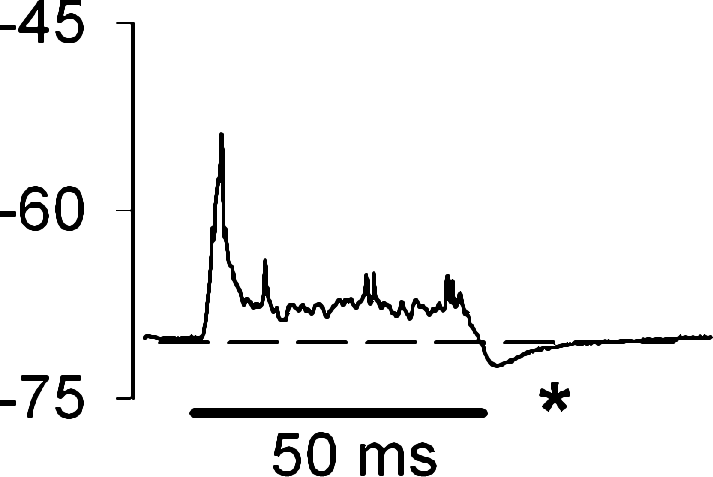
\includegraphics{TStellate/OC-99-812-013}}}
\caption[Average intracelluar response data in stellate cells in rats.]{Average
  intracelluar response to CF tone 30dB above depolarisation threshold in
  stellate
  cells~\citep[Reproduced~from~][]{PaoliniClareyEtAl:2005}. A. Sustained chopper
  unit 01-864-004. B. Transient chopper type 1 unit 01-857-007, CF
  8.9kHz. C. Transient chopper type 2 unit 01-305-014. D. Onset chopper unit
  99-812-013. Hyperpolarisation after tone indicated by
  asterix.  \label{fig:PaoliniAIV}}
\end{figure}

\yellownote{Permission needed for Paolini plots}


\begin{figure}[htb]
  \centering
  \resizebox{0.5\textwidth}{!}{\includegraphics{TStellate/PaoliniCV.eps}}
  \caption{Regularity in chopper units \citep[Data reproduced from Fig.~2,~][]{PaoliniClareyEtAl:2005}}
  \label{fig:PaoliniCVdata}
\end{figure}





\subsection{Implementation}

\yellownote{Para 1: Nordlie table~\ref{tab:TSModelSummary}A. Using R\&M type 1-t, Other previous models}


\yellownote{Synaptic inputs known and unknown, included and not included in model.  Previous work include and excludes}



Figure~\ref{fig:TSinputs} shows the expected response of a T~stellate cell to
individual connections from different cell types. The membrane parameters for
the single compartment T~stellate cell model are default except for sodium
conductance set to zero. In this example, excitation from the afferent
\ANF~inputs (\LSR~Figure~\ref{fig:TSinputs}A and
\HSR~Figure~\ref{fig:TSinputs}B) show a large depolarisation.  \HSR~inputs show
a rapid onset and a slowly adapting sustained depolarisation.


\yellownote{Actual parameters: diameter =19.5$\mu$m, $\bar{g}_{\rm Na}=0$,
$\bar{g}_{\rm KHT}=0.0189416$ S cm$^{-2}$, $\bar{g}_{\rm leak}=0.000473539$ S
cm$^{-2}$, $\bar{g}_{\rm h}=6.20392e-05$ S cm$^{-2}$, $\bar{g}_{\rm KA}=0.01539$
S cm$^{-2}$,E$_{\rm rev}=-65$ mV, E$_{\rm Na}=50$ mV, E$_{\rm K}=-70$ mV.}  


\begin{figure}[htb]
  \centering
  \resizebox{0.6\textwidth}{!}{\includegraphics{TStellate/baseline_exc}}
  \resizebox{0.6\textwidth}{!}{\includegraphics{TStellate/baseline_inh}}
  \caption[Response of T~stellate cells to isolated synaptic
  inputs]{Intracellular membrane voltage response of a T~stellate cell model to
    isolated synaptic inputs. A pure tone stimulus of 8.2~kHz at 85 dB~SPL was
    presented to the CN network. The CF of the recorded T~stellate cell was
    8.267~kHz.  Single stimulus responses are shown as a thin line and average
    response over 25 repetitions is shown as the dark line. A. 30 LSR ANF
    synapses. B. 20 HSR ANF synapsexs. C. 20 D stellate cell glycinergic
    synapses. D. 15 Golgi cell GABA$_{\rm A}$ synapses. All weights were set to
    $0.0005\,\mu{\rm S}$ and the sodium conductance set to zero.  The parameters
    for synapases were: excitatory (tau = 0.36 msec), glycinergic (tau1=0.4 and
    tau2=2.5 msec), and GABAergic (tau1=0.26 and tau2=5.43
    msec).\label{fig:TSinputs}}
\end{figure}

\begin{figure}[htb]
  \centering
  \resizebox{0.6\textwidth}{!}{\includegraphics{TStellate/baseline_exc}}
  \resizebox{0.6\textwidth}{!}{\includegraphics{TStellate/baseline_jitter.eps}}
\caption[Response of T~stellate cells to isolated synaptic
  inputs]{Intracellular membrane voltage response of a T~stellate cell model to
    isolated synaptic inputs. A pure tone stimulus of 8.2~kHz at 85 dB~SPL was
    presented to the CN network. The CF of the recorded T~stellate cell was
    8.267~kHz.  Single stimulus responses are shown as a thin line and average
    response over 25 repetitions is shown as the dark line. A. 30 LSR ANF
    synapses. B. 20 HSR ANF synapsexs. C. 20 D stellate cell glycinergic
    synapses. D. 15 Golgi cell GABA$_{\rm A}$ synapses. All weights were set to
    $0.0005\,\mu{\rm S}$ and the sodium conductance set to zero.  The parameters
    for synapases were: excitatory (tau = 0.36 msec), glycinergic (tau1=0.4 and
    tau2=2.5 msec), and GABAergic (tau1=0.26 and tau2=5.43
    msec).\label{fig:TSExcinputs}}
%  \caption[]{Jitter of AN input T~stellate Optimisation results}
%  \label{fig:CSjitter}
\end{figure}





\subsection{Optimisation Results}

Choosing optimisation data - average population data or individual exemplar based on Paolini rat data.


What is not shown in Figure~\ref{fig:TSinputs} is firstly the non-linear
dynamics of the action potential in the neural model; and secondly the
hyperpolarisation activation of I$_{\rm h}$ and I$_{\rm KA}$ currents due to inhibitory
input.  The second factor is important in enhancing the first spike response
across the T~stellate cells \citep{PaoliniClareyEtAl:2004}to an oncoming
stimulus, since the \OnC~units will respond earlier and provide fast inhibition 

%       \begin{figure}[htb]
%         \centering\resizebox{0.95\textwidth}{!}{%
%           \includegraphics{RateLevel/psthsingle90.0.eps}%
% %          \includegraphics{RateLevel/TS_ratelevel.eps}}
%       \end{figure}



\subsubsection{Sustained chopper}


\subsubsection{Transient Chopper}
\begin{figure}[htb]
  \centering
  \resizebox{0.6\textwidth}{!}{\includegraphics{TStellate_CT1/plot.eps}}
  \caption[CT1 T~stellate Optimisation results]{CT1 T~stellate Optimisation results}
  \label{fig:CT1results}
\end{figure}

\begin{figure}[htb]
  \centering
  \resizebox{0.6\textwidth}{!}{\includegraphics{TStellate_CT2/plot.eps}}
  \caption[CT2 T~stellate Optimisation results]{CT2 T~stellate Optimisation results}
  \label{fig:CT2results}
\end{figure}



{\small% % D~----------------------------------
\noindent\begin{tabularx}{\linewidth}{|X|c|c|c|c|c|}
\hdr{6}{F}{Optimisation} \\ \hline
       \textbf{Parameters}         &    \textbf{Name}     & \textbf{Range} & \multicolumn{3}{|c|}{\textbf{Best Values}} \\
                                   &                      &                & CS&     CT1     & CT2 \\\hline
Weight of HSR syn on TS  ($\mu$S)  &       \wHSRTS        &  [1e-5,0.03]   &   & 0.000708301 & 0.00168911\\
Weight of LSR syn on TS  ($\mu$S)  &       \wLSRTS        &  [1e-5,0.03]   &   &  (0.0025)   & 0.00140628\\
 %  Number of synapses, LSR to TS  &       \nLSRTV        &     [0,64]     &   &             & \\
 %  Number of synapses, HSR to TS  &       \nHSRTV        &     [0,64]     &   &             & \\
 Weight of DS syn on TS  ($\mu$S)  &        \wDSTS        &  [1e-5,0.03]   &   &      --      & --\\
%Number of DS syn on TS  ($\mu$S)  &        \nDSTS        &     [0,64]     &   &             & \\
 Weight of TV syn on TS  ($\mu$S)  &        \wTVTS        &  [1e-5,0.03]   &   &      --      & --\\
%Number of TV syn on TS  ($\mu$S)  &        \nTVTS        &     [0,64]     &   &             & \\
Weight of GLG syn on TS  ($\mu$S)  &       \wGLGTS        &  [1e-5,0.03]   &   &      --      & --\\
%Number of GLG syn on TS  ($\mu$S) &       \nGLGTS        &     [0,64]     &   &             & \\ \hline
 TS~leak conductance (S cm$^{-2}$)  & $\bar{g}_{\rm leak}$ &  [1e-6,0.003]  &   & 0.000860145 & 8.9326e-05\\ 
 TS~KHT conductance (S cm$^{-2}$)   & $\bar{g}_{\rm KHT}$  &  [1e-6,0.003]  &   &  (0.0189)   & 0.0226787\\ 
  TS~reversal potential (mV)     &    E$_{\rm rev}$     &   [-45,-70]    &   &   -54.26    & -63.502\\ \hline
                       \multicolumn{3}{|l|}{Error}                         &   &   11.886    & 31.481\\ \hline 
\end{tabularx}
}




\section{Verification}

\subsection{Effect of DS: time frequency enhancement}

Go on Paolini's proposal

\subsection{Effect of TV: comb filter and echo suppression}


%       \subsection{Tone Response}

%       \begin{figure}[htb]
%         \centering\resizebox{0.95\textwidth}{!}{%
%           \includegraphics{RateLevel/psthsingle90.0.eps}%
% %          \includegraphics{RateLevel/TS_ratelevel.eps}}
%       \end{figure}
%       \begin{figure}[htb]
%         \centering\resizebox{0.95\textwidth}{!}{%
%  %         \includegraphics{RateLevel/response_area.0.eps}%
%   %        \includegraphics{RateLevel/response_area_log2.0.eps}}
%       \end{figure}
%       \begin{figure}[htb]
%         \centering\resizebox{0.95\textwidth}{!}{%
%           % \includegraphics{RateLevel/response_area.0.eps}
%           \includegraphics{RateLevel/psthall90.0.eps}%
%           \includegraphics{RateLevel/psthVlevel.0.eps}}
%       \end{figure}


%       \clearpage
%       \subsection{Noise Response}
%       \begin{figure}[htb]
%         \centering\resizebox{0.95\textwidth}{!}{%
%           \includegraphics{NoiseRateLevel/psthsingle120.0.eps}%
%           \includegraphics{NoiseRateLevel/TS_ratelevel.eps}}
%       \end{figure}
%       \begin{figure}[htb]
%         \centering\resizebox{0.95\textwidth}{!}{%
%           \includegraphics{NoiseRateLevel/response_area.0.eps}%
%           \includegraphics{NoiseRateLevel/response_area_log2.0.eps}}
%       \end{figure}
%       \begin{figure}[htb]
%         \centering\resizebox{0.95\textwidth}{!}{%
%           % \includegraphics{RateLevel/response_area.0.eps}
%           \includegraphics{NoiseRateLevel/psthall90.0.eps}%
%           \includegraphics{NoiseRateLevel/psthVlevel.0.eps}}
%       \end{figure}


%       \clearpage
%       \subsection{Masked Noise and Tone}
%       \begin{figure}[h!]
%         \centering\resizebox{0.95\textwidth}{!}{\includegraphics{MaskedRateLevel/psthsingle90.0.eps}\includegraphics{MaskedRateLevel/TS_ratelevel.eps}}
%       \end{figure}
%       \begin{figure}[h!]
%         \centering\resizebox{0.95\textwidth}{!}{%
%           \includegraphics{MaskedRateLevel/response_area.0.eps}%
%           \includegraphics{MaskedRateLevel/response_area_log2.0.eps}}
%       \end{figure}

%       \begin{figure}[h!]
%         \centering\resizebox{0.95\textwidth}{!}{%
%           % \includegraphics{RateLevel/response_area.0.eps}
%           \includegraphics{MaskedRateLevel/psthall90.0.eps}%
%           \includegraphics{MaskedRateLevel/psthVlevel.0.eps}}
%       \end{figure}
%       \clearpage
%       \subsection{Masked Response Area}
%       \begin{figure}[h!]
%         \centering\resizebox{0.95\textwidth}{!}{%
%           \includegraphics{MaskedResponseCurve/psthsingle5810.0.eps}%
%           \includegraphics{MaskedResponseCurve/TS_masked.eps}}
%       \end{figure}
%       \begin{figure}[h!]
%         \centering\resizebox{0.95\textwidth}{!}{%
%           \includegraphics{MaskedResponseCurve/response_area.0.eps}%
%           \includegraphics{MaskedResponseCurve/response_area_log2log2.0.eps}}
%       \end{figure}

%       \begin{figure}[h!]
%         \centering\resizebox{0.95\textwidth}{!}{%
%           % \includegraphics{RateLevel/response_area.0.eps}
%           \includegraphics{MaskedResponseCurve/psthall5810.0.eps}%
%           \includegraphics{MaskedResponseCurve/psthVmod.0.eps}}
%       \end{figure}
%       \clearpage





      % \todo{add stuff here}



      % %%%%%%%%%%%%%%%%%%%%%%%%%%%%%%%%%%%%%%%%%%%%%%%%%%%%%% 
    %   \bibliographystyle{plainnat}%bmc_article} % Style BST file
    %   \bibliography{../hg/manuscript/bib/MyBib}
      
    % \end{document}


%%% Local Variables: 
%%% mode: latex
%%% mode: tex-fold
%%% TeX-master: "SimpleResponses"
%%% TeX-PDF-mode: nil
%%% End: 
